\section{Programmable logic device}

The behaviour that I tried to emulate by means of the FPGA consists in reading the status of a group of buttons and send them to the microcontroller via single wire communication protocol: UART. So, the overall architecture is composed of two main parts:
\begin{itemize}
\item The logic of interface for the keyboard
\item UART peripheral VHDL-based (only TX channel). It will be described in the next section
\end{itemize}

\begin{figure}[H]
\centering
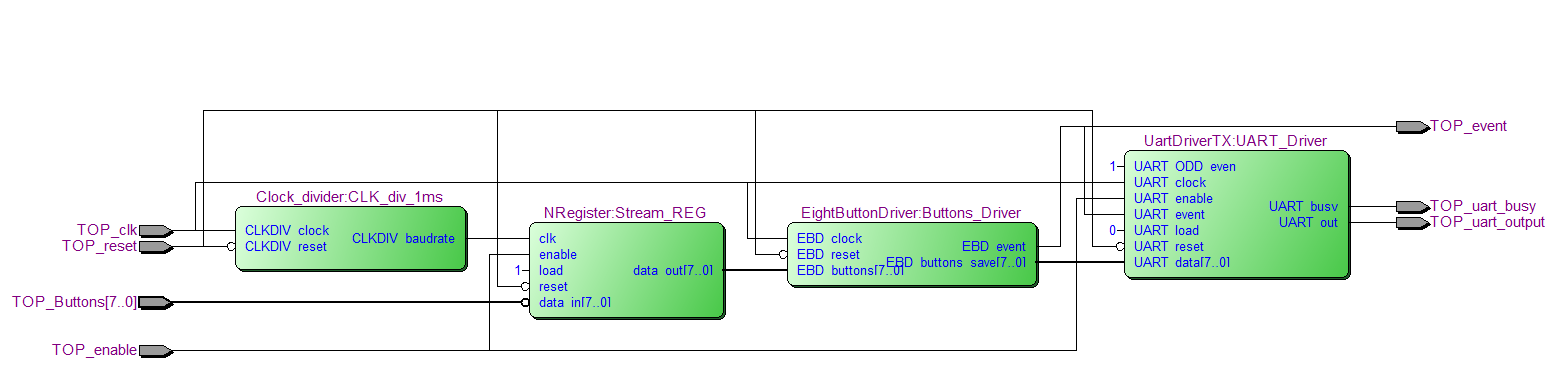
\includegraphics[scale=.5]{Immagini/15}
\label{15}
\caption{Top level entity view}
\end{figure}

Clock is internally generated by the FPGA at 50 MHz, however in some point of the architecture I needed to slow down. The clock feeding the output shift register within UART peripheral block runs at 115400 bit/s around. Another clock divider is used to sample buttons each 1 ms. During my tests, I noticed that the architecture worked well in simulation, but scoping the UART output with an oscilloscope probe I saw the mess. This totally uncorrect behaviour was given by the fact that button are mechanical objects generating a bouncing signal when pushed. So I measured the duration of these oscillations, leading me at the conclusion of implementing a "debouncing logic", in my project composed of a register and a clock divisor, the ones are shown in the top level entity view. The input signals got stable after some hundreds of $\mu s$, until $800 \mu s$ in some cases. That's the reason why I perform input sampling each one millisecond. I'm sure that in this interval oscillations expire.
\newline
\newline
Clock dividers I implemented are both fed by the 50 Mhz clock. Internally the output of a counter is compared with the one contained within an hardwired register. The comparator performs the equality checking operation. Every time comparison gets true, the counter is reset in next cycle. 
 The output of clock divider is the one of the comparator; in such a way the resulting waveform is a train of pulses having the desired baudrate.
 \begin{figure}[H]
\centering
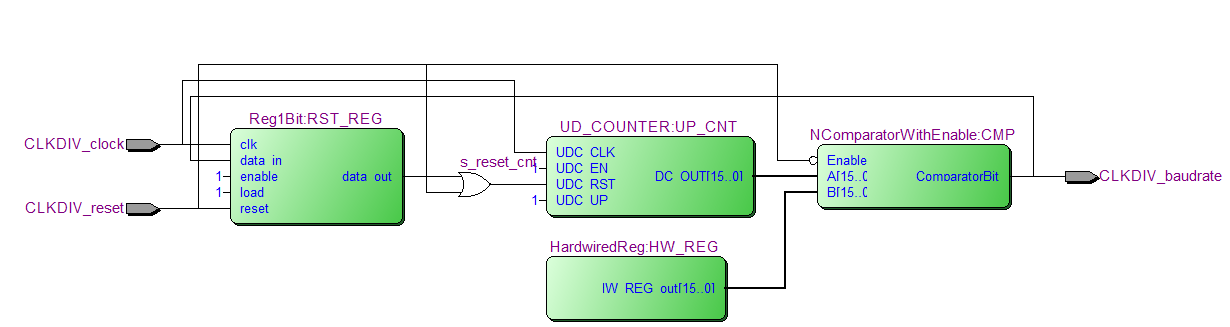
\includegraphics[scale=.6]{Immagini/17}
\label{17}
\caption{Clock divider architecture}
\end{figure}
 \begin{figure}[H]
\centering
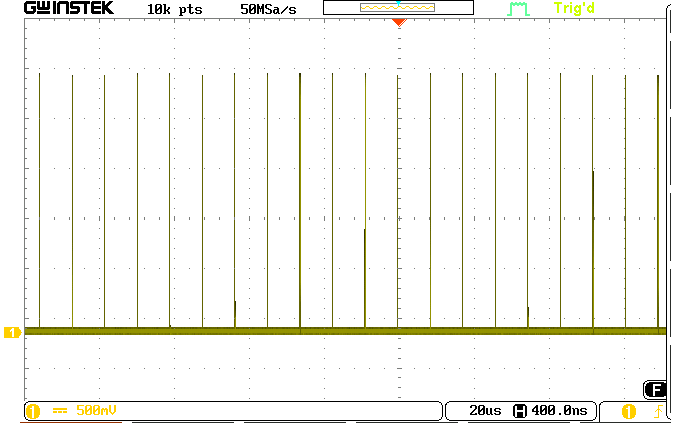
\includegraphics{Immagini/16}
\label{16}
\caption{Clock divider output within UART peripheral. Time between two consecutive pulses is $9 \mu s$, leading a baudrate of 115200 bit/s. The hardwired value is 434, from the round division between 50Mhz and 115200 Hz}
\end{figure}

The eight buttons driver just simply recognizes when a button has been pushed and generates an "event", then sent to the UART peripheral to start the transfer. Two registers are on the output, one for buttons, one for the event bit.
\newline
\newline
I'm going to talk about UART peripheral implementation in the next section, dedicated to \textbf{Interconnection protocol}. Another VHDL component, that is not integrated here, is the memory controller for the SDRAM laid on the Altera board; the last section \textbf{Memory management} is dedicated to it and some comparisons between waveform simulation and real required access protocol will be shown.

 \begin{figure}[H]
\centering
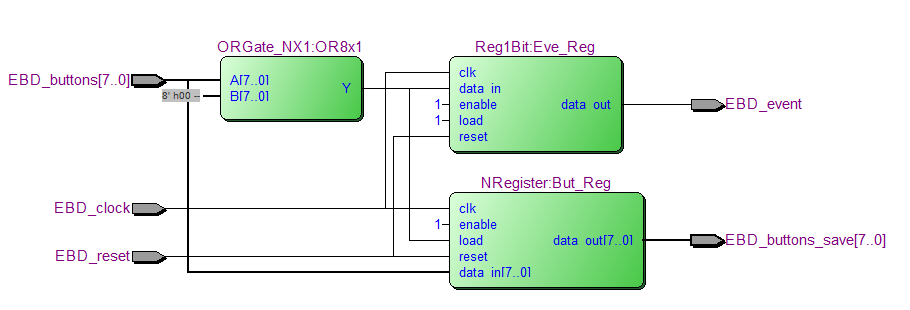
\includegraphics[scale=.8]{Immagini/18}
\label{18}
\caption{Eight button driver architecture}
\end{figure}

\begin{table}[H]
\centering
\begin{tabular}{p{0.3\textwidth}p{0.2\textwidth}p{0.3\textwidth}}

\textbf{Node name}&\textbf{Direction}&\textbf{Location}\\ \hline
TOP\_reset & Input & J15 (Push Button[0])\\
TOP\_enable& Input & M1 (DIP\_switch[0])\\
TOP\_clk	&Input & R8 (Internal clock source 50 Mhz)\\
TOP\_buttons[0]	& Input & D5 (GPIO\_09)\\ 
TOP\_buttons[1]	& Input & A6 (GPIO\_011)\\ 
TOP\_buttons[2]	& Input & D6 (GPIO\_013)\\ 
TOP\_buttons[3]	& Input & C6 (GPIO\_015)\\ 
TOP\_buttons[4]	& Input & E6 (GPIO\_017)\\ 
TOP\_buttons[5]	& Input & D8 (GPIO\_019)\\ 
TOP\_buttons[6]	& Input & F8 (GPIO\_021)\\ 
TOP\_buttons[7]	& Input & E9 (GPIO\_023)\\ 
TOP\_uart\_output & Output & D3 (GPIO\_00)\\
TOP\_uart\_busy	  & Output & C3 (GPIO\_01), not used, just for debugging\\
TOP\_event		& Output	& A3 (GPIO\_03), not used, just for debugging\\
\hline
\end{tabular}
\caption{FPGA pin assignment}
\end{table}

\begin{figure}[H]
\centering
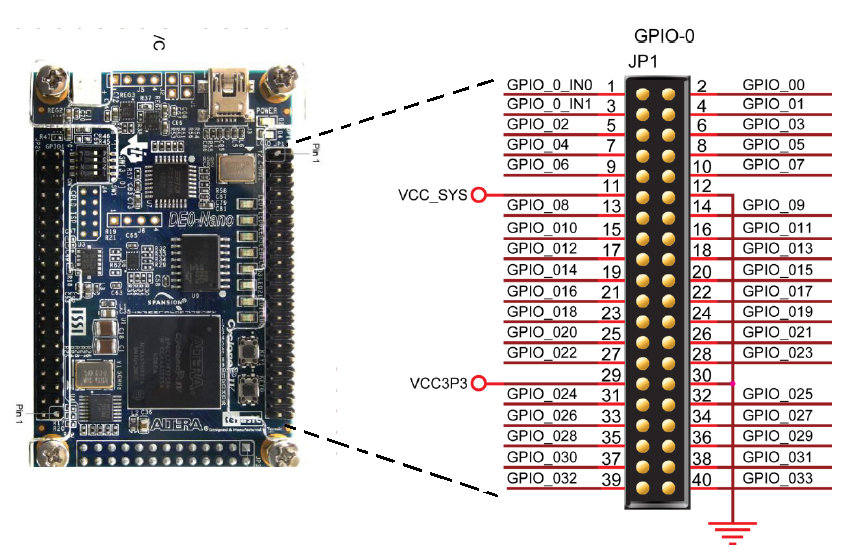
\includegraphics[scale=.8]{Immagini/19}
\label{19}
\caption{Altera DE0 Nano GPIO pinout}
\end{figure}